\def\baselinestretch{1}
\chapter{Applicazione realizzata} \label{cap3}
\def\baselinestretch{1.66}
\noindent Il progetto di tesi proposto ha come focus principale la realizzazione del docking tra i ligandi contenuti in specifici pesticidi e i recettori dell'apis mellifera e l'estrazione dei legami che si vengono a formare. Il software realizzato può essere utilizzato in due modalità: mediante script python da terminale o mediante interfaccia grafica. 

\section{Dati in input}
\def\baselinestretch{1.66}
\noindent I dati in input all'applicazione trattata sono: ligandi e proteine. La lista dei ligandi è fornita in input tramite foglio calcolo (.xlsx, .xls) o mediante file di testo (.txt), in entrambi i casi ogni riga corrisponde al nome di un ligando. Essendo l'applicazione incentrata sullo studio degli effetti dei ligandi dei pesticidi sull'apis mellifera, come dati di esempio sono state utilizzati i ligandi le cui molecole costituiscono i pesticidi maggiormente diffusi 
sul mercato %inserire tabella con lista dei pesticidi.
per un totale di 297 ligandi. La lista è disponibile nell'appendice \ref{tab:Tabella dei Ligandi}.\newline
I recettori vengono selezionati mediante una web view aperta sulla pagina di ricerca del sito di \textbf{PubChem}, l'utente digiterà la propria query e dopo aver selezionato il tasto \textit{research} gli verranno mostrati tutti i composti organici relativi alla query digitata, tramite il tasto \textit{Get Query} l'utente andrà a scaricare tutti i file dei composti organici in formato .pdb. Nel caso di esempio sono state scelte tutte le proteine dei recettori dell'Apis Mellifera come mostrato nelle foto: \ref{fig:queryRecettori} e \ref{fig:fileRecettori}, per un totale di 60 file .pdb contenenti le strutture di determinate proteine.
\begin{figure}[H]
    \centering
    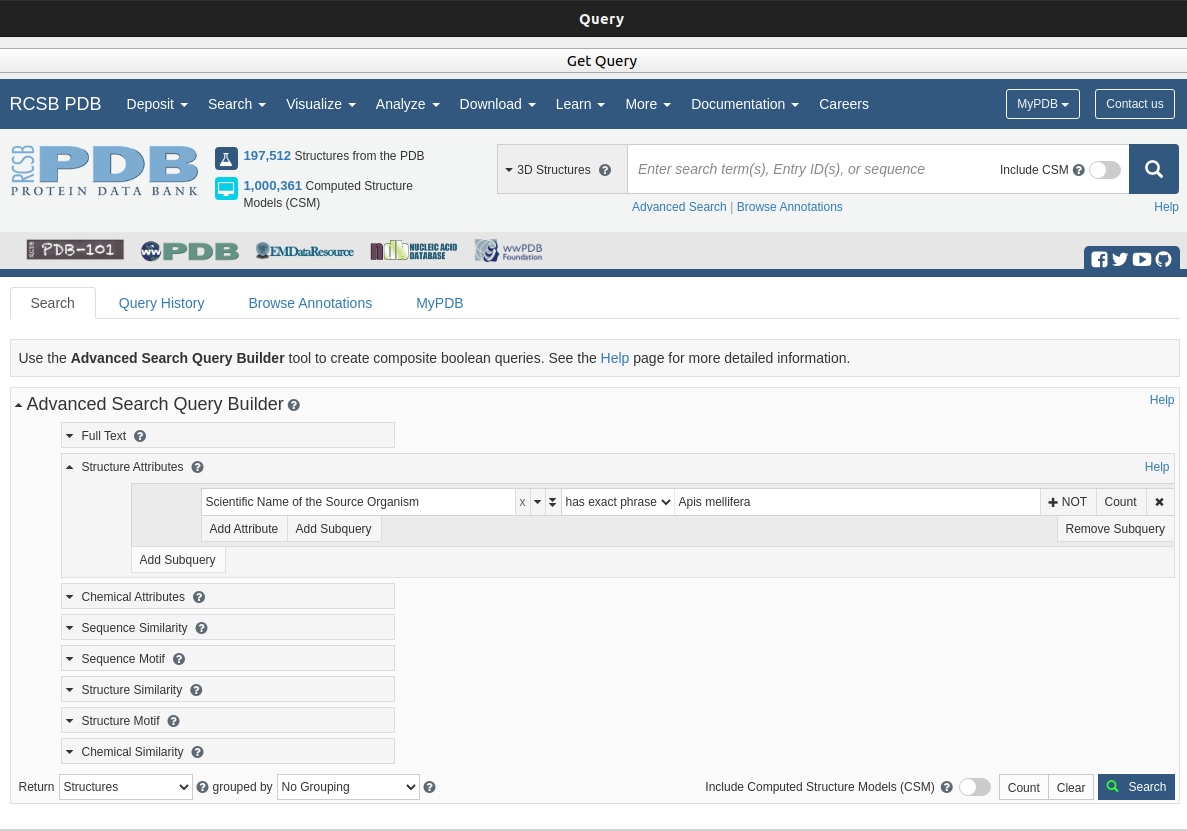
\includegraphics[scale=0.4]{immagini/queryRecettori.png}
    \caption{Query dei recettori}
    \label{fig:queryRecettori}
\end{figure}

\begin{figure}[H]
    \centering
    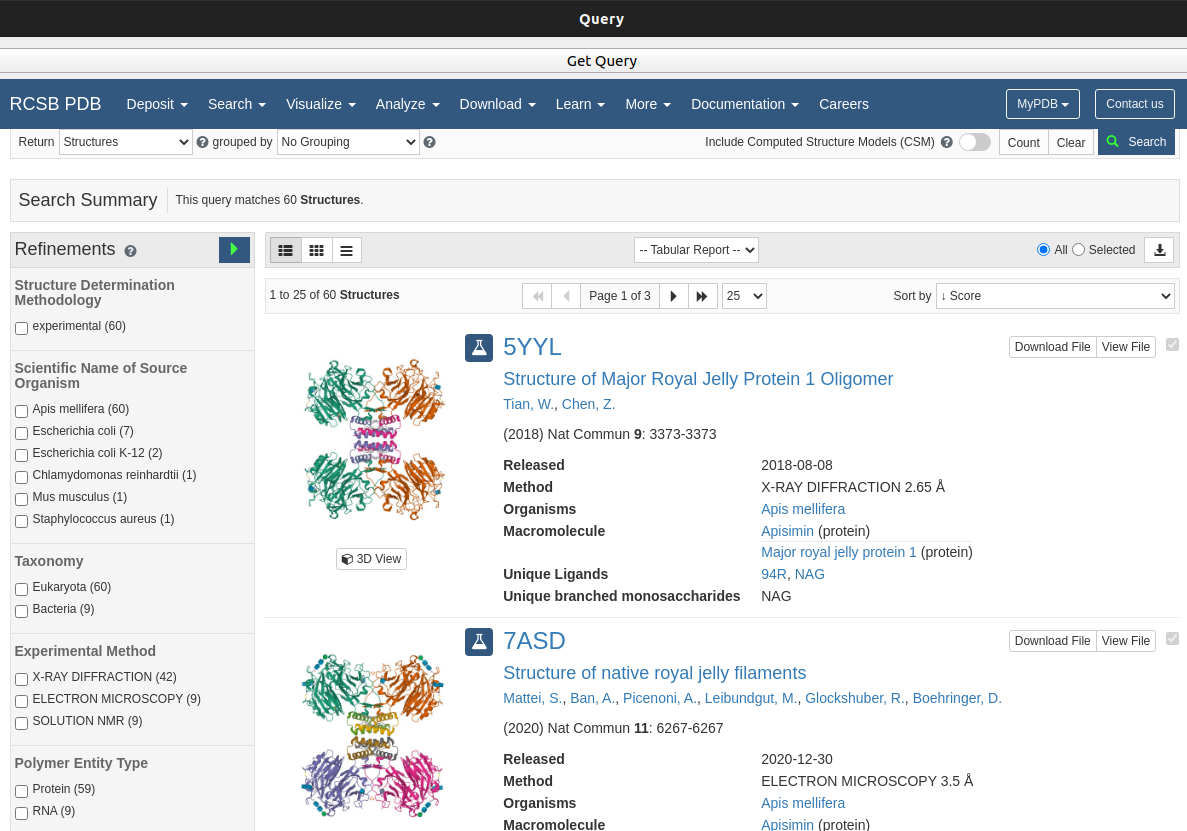
\includegraphics[scale=0.4]{immagini/fileRecettori.png}
    \caption{Proteine dei recettori dell'apis mellifera}
    \label{fig:fileRecettori}
\end{figure}

\section{Preparazione dei ligandi e dei recettori}
\def\baselinestretch{1.66}
\noindent Il primo step propedeutico per il docking è la preparazione dei ligandi e dei recettori, questa
fase viene esplicitamente eseguita dal software realizzato.

\subsection{Preparazione dei ligandi}
\noindent La lista di ligandi da scaricare è fornita in input mediante un file di testo (.txt) alla nostra applicazione o mediante foglio di calcolo (.xlsx, .xls), all'interno della lista sono presenti i nomi dei ligandi uno sotto all'altro. Tramite la funzione